% --------------------------------------------------
% 
% This chapter is for dingo
% 
% --------------------------------------------------

\chapter{Software development to establish metabolic flux sampling 
         approaches at the community level}
\label{cha:dingo}

% ADD AN INTRO FOR THE SECTION

\section{Genome-scale metabolic model analysis}

The relationship between genotype and phenotype is fundamental to biology.
Many levels of control are introduced when moving from one to the other. 
Systems biology aims at deciphering "the strategy" both at the cell and at higher levels of organization, in case of multicell species, that enables organisms to produce orderly adaptive behavior in the face of widely varying genetic and environmental conditions (\cite{strohman2002maneuvering}); the term "strategy" is used as per \cite{polanyi1968life}.
Systems biology approaches aim at interpreting how a system's properties emerge; from the cell to the community level.


\section{A New MCMC Algorithm for Sampling the Flux Space of Metabolic Networks}


\cite{chalki2021SoCG}

% \section{The flux sampling approach}

From \citet{price2004genome} :
"Pairwise correlation coefficients can be calculated
between all reaction fluxes based on uniform random
sampling. Perfectly correlated reactions (R2 = 1) operate
as functional modules within a biochemical network,
whereas uncorrelated reactions (R2 ~0) operate independently of each other. The degree of independence
between reactions is an important consideration when
choosing a set of fluxes to measure that will best determine the operating state of a biochemical network"


Write something from \citeauthor{polanyi1968life}

% \section{The `dingo` Python library}


our approach 

\begin{figure}
   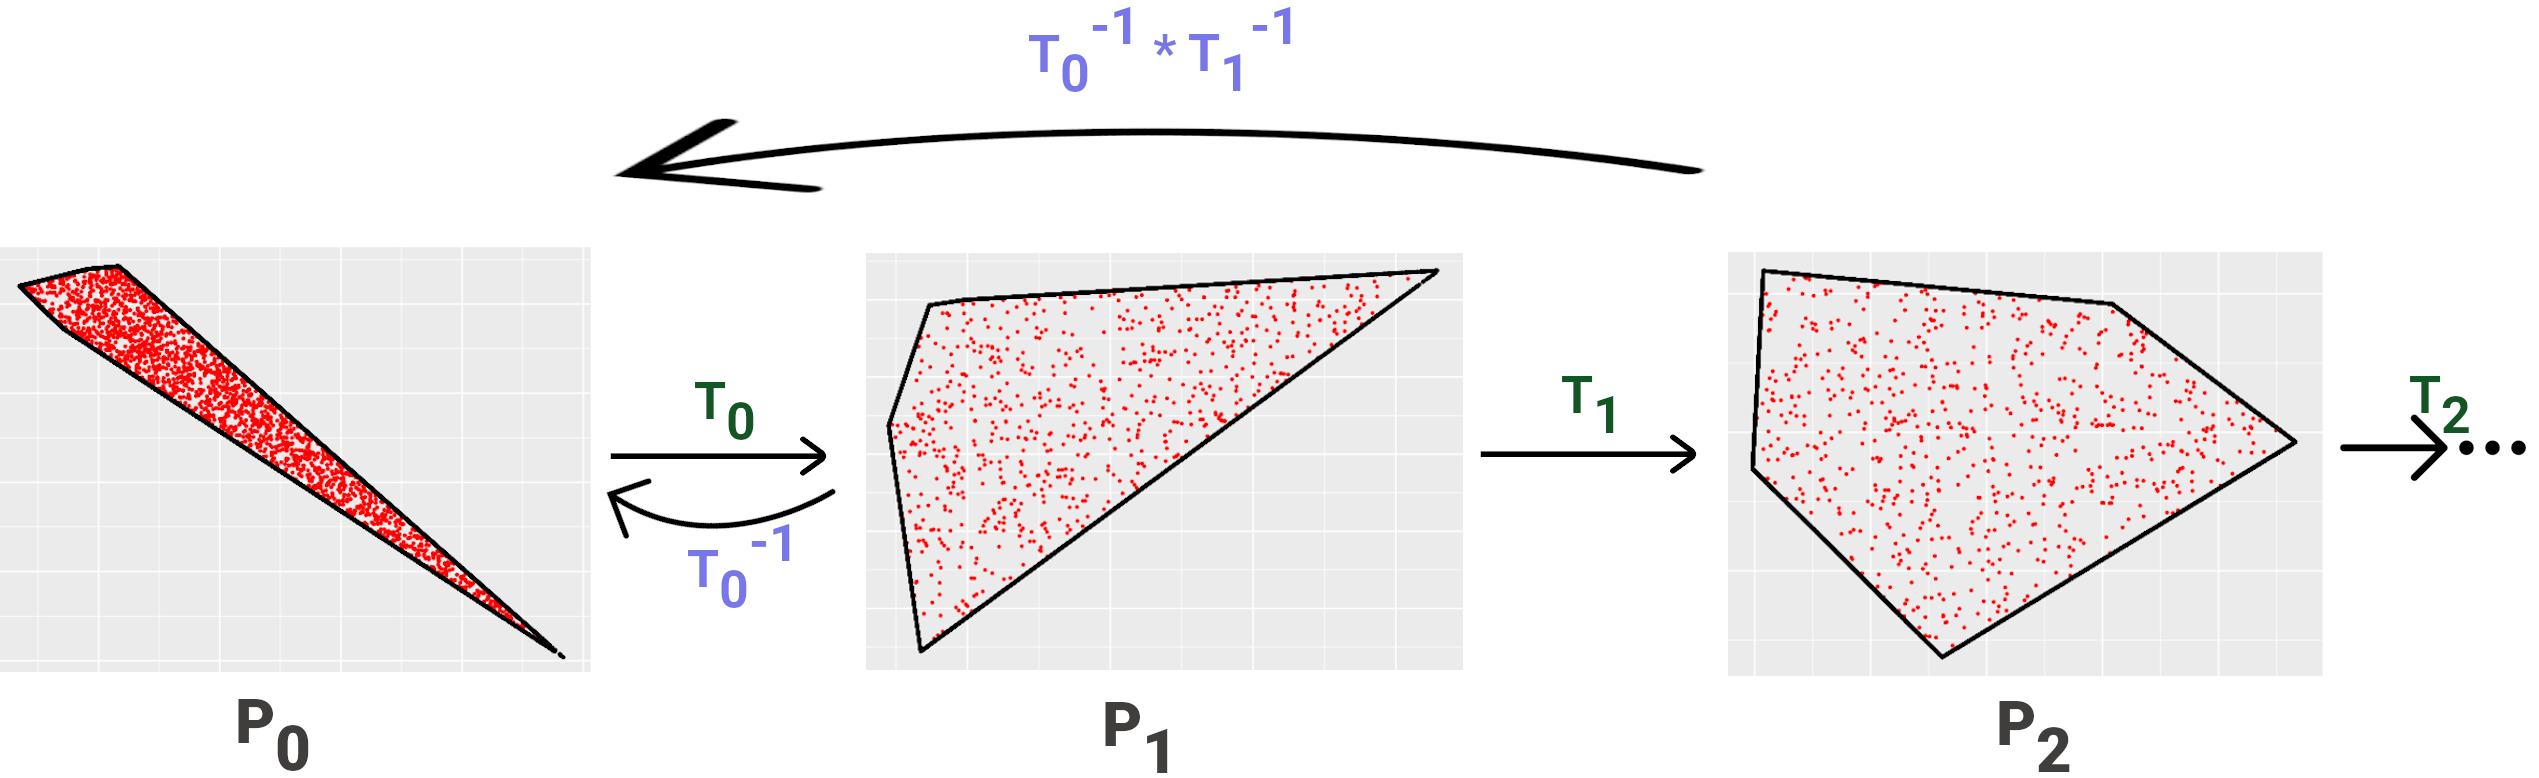
\includegraphics[width=1.0\columnwidth]{figures/sampling_extra_phase_croped.png}
   \caption{Our MMCS algorithm and its first phases}
   \label{fig:mmcs}
\end{figure}


% SECTION 3
\section{Flux sampling at the community level}



%%% Local Variables: 
%%% mode: latex
%%% TeX-master: "thesis"
%%% End: 
